%%%%%%%%%%%%%%%%%%%%%%%%%%%%%%%%%%%%%%%%%
% Wenneker Article
% LaTeX Template
% Version 2.0 (28/2/17)
%
% This template was downloaded from:
% http://www.LaTeXTemplates.com
%
% Authors:
% Vel (vel@LaTeXTemplates.com)
% Frits Wenneker
%
% License:
% CC BY-NC-SA 3.0 (http://creativecommons.org/licenses/by-nc-sa/3.0/)
%
%%%%%%%%%%%%%%%%%%%%%%%%%%%%%%%%%%%%%%%%%

%----------------------------------------------------------------------------------------
%	PACKAGES AND OTHER DOCUMENT CONFIGURATIONS
%----------------------------------------------------------------------------------------
\documentclass[10pt, a4paper, twocolumn]{article} % 10pt font size (11 and 12 also possible), A4 paper (letterpaper for US letter) and two column layout (remove for one column)

\usepackage{hyperref}

%%%%%%%%%%%%%%%%%%%%%%%%%%%%%%%%%%%%%%%%%
% Wenneker Article
% Structure Specification File
% Version 1.0 (28/2/17)
%
% This file originates from:
% http://www.LaTeXTemplates.com
%
% Authors:
% Frits Wenneker
% Vel (vel@LaTeXTemplates.com)
%
% License:
% CC BY-NC-SA 3.0 (http://creativecommons.org/licenses/by-nc-sa/3.0/)
%
%%%%%%%%%%%%%%%%%%%%%%%%%%%%%%%%%%%%%%%%%

%----------------------------------------------------------------------------------------
%	PACKAGES AND OTHER DOCUMENT CONFIGURATIONS
%----------------------------------------------------------------------------------------

\usepackage[english]{babel} % English language hyphenation

\usepackage{microtype} % Better typography

\usepackage{amsmath,amsfonts,amsthm} % Math packages for equations

\usepackage[svgnames]{xcolor} % Enabling colors by their 'svgnames'

\usepackage[hang, small, labelfont=bf, up, textfont=it]{caption} % Custom captions under/above tables and figures

\usepackage{booktabs} % Horizontal rules in tables

\usepackage{lastpage} % Used to determine the number of pages in the document (for "Page X of Total")

\usepackage{graphicx} % Required for adding images

\usepackage{enumitem} % Required for customising lists
\setlist{noitemsep} % Remove spacing between bullet/numbered list elements

\usepackage{sectsty} % Enables custom section titles
\allsectionsfont{\usefont{OT1}{phv}{b}{n}} % Change the font of all section commands (Helvetica)

%----------------------------------------------------------------------------------------
%	MARGINS AND SPACING
%----------------------------------------------------------------------------------------

\usepackage{geometry} % Required for adjusting page dimensions

\geometry{
	top=1cm, % Top margin
	bottom=1.5cm, % Bottom margin
	left=2cm, % Left margin
	right=2cm, % Right margin
	includehead, % Include space for a header
	includefoot, % Include space for a footer
	%showframe, % Uncomment to show how the type block is set on the page
}

\setlength{\columnsep}{7mm} % Column separation width

%----------------------------------------------------------------------------------------
%	FONTS
%----------------------------------------------------------------------------------------

\usepackage[T1]{fontenc} % Output font encoding for international characters
\usepackage[utf8]{inputenc} % Required for inputting international characters

\usepackage{XCharter} % Use the XCharter font

%----------------------------------------------------------------------------------------
%	HEADERS AND FOOTERS
%----------------------------------------------------------------------------------------

\usepackage{fancyhdr} % Needed to define custom headers/footers
\pagestyle{fancy} % Enables the custom headers/footers

\renewcommand{\headrulewidth}{0.0pt} % No header rule
\renewcommand{\footrulewidth}{0.4pt} % Thin footer rule

\renewcommand{\sectionmark}[1]{\markboth{#1}{}} % Removes the section number from the header when \leftmark is used

%\nouppercase\leftmark % Add this to one of the lines below if you want a section title in the header/footer

% Headers
\lhead{} % Left header
\chead{\textit{\thetitle}} % Center header - currently printing the article title
\rhead{} % Right header

% Footers
\lfoot{} % Left footer
\cfoot{} % Center footer
\rfoot{\footnotesize Page \thepage\ of \pageref{LastPage}} % Right footer, "Page 1 of 2"

\fancypagestyle{firstpage}{ % Page style for the first page with the title
	\fancyhf{}
	\renewcommand{\footrulewidth}{0pt} % Suppress footer rule
}

%----------------------------------------------------------------------------------------
%	TITLE SECTION
%----------------------------------------------------------------------------------------

\newcommand{\authorstyle}[1]{{\large\usefont{OT1}{phv}{b}{n}\color{DarkRed}#1}} % Authors style (Helvetica)

\newcommand{\institution}[1]{{\footnotesize\usefont{OT1}{phv}{m}{sl}\color{Black}#1}} % Institutions style (Helvetica)

\usepackage{titling} % Allows custom title configuration

\newcommand{\HorRule}{\color{DarkGoldenrod}\rule{\linewidth}{1pt}} % Defines the gold horizontal rule around the title

\pretitle{
	\vspace{-30pt} % Move the entire title section up
	\HorRule\vspace{10pt} % Horizontal rule before the title
	\fontsize{32}{36}\usefont{OT1}{phv}{b}{n}\selectfont % Helvetica
	\color{DarkRed} % Text colour for the title and author(s)
}

\posttitle{\par\vskip 15pt} % Whitespace under the title

\preauthor{} % Anything that will appear before \author is printed

\postauthor{ % Anything that will appear after \author is printed
	\vspace{10pt} % Space before the rule
	\par\HorRule % Horizontal rule after the title
	\vspace{20pt} % Space after the title section
}

%----------------------------------------------------------------------------------------
%	ABSTRACT
%----------------------------------------------------------------------------------------

\usepackage{lettrine} % Package to accentuate the first letter of the text (lettrine)
\usepackage{fix-cm}	% Fixes the height of the lettrine

\newcommand{\initial}[1]{ % Defines the command and style for the lettrine
	\lettrine[lines=3,findent=4pt,nindent=0pt]{% Lettrine takes up 3 lines, the text to the right of it is indented 4pt and further indenting of lines 2+ is stopped
		\color{DarkGoldenrod}% Lettrine colour
		{#1}% The letter
	}{}%
}

\usepackage{xstring} % Required for string manipulation

\newcommand{\lettrineabstract}[1]{
	\StrLeft{#1}{1}[\firstletter] % Capture the first letter of the abstract for the lettrine
	\initial{\firstletter}\textbf{\StrGobbleLeft{#1}{1}} % Print the abstract with the first letter as a lettrine and the rest in bold
}

%----------------------------------------------------------------------------------------
%	BIBLIOGRAPHY
%----------------------------------------------------------------------------------------

\usepackage[backend=bibtex,style=numeric,natbib=true]{biblatex} % Use the bibtex backend with the authoryear citation style (which resembles APA)

\addbibresource{example.bib} % The filename of the bibliography

\usepackage[autostyle=true]{csquotes} % Required to generate language-dependent quotes in the bibliography
 % Specifies the document structure and loads requires packages
%----------------------------------------------------------------------------------------
%	ARTICLE INFORMATION
%----------------------------------------------------------------------------------------

\title{ByWire Trust Indicator} % The article title

\author{
	\authorstyle{Jetze Sikkema\textsuperscript{1}} % Authors
	\newline\newline % Space before institutions
	\textsuperscript{1}\institution{\href{http://bywire.news}{ByWire, 35 Little Russell St, London, United Kingdom}} \\ % Institution 1
}

% Example of a one line author/institution relationship
%\author{\newauthor{John Marston} \newinstitution{Universidad Nacional Autónoma de México, Mexico City, Mexico}}

\date{\today} % Add a date here if you would like one to appear underneath the title block, use \today for the current date, leave empty for no date

%----------------------------------------------------------------------------------------

\begin{document}

\maketitle % Print the title

\thispagestyle{firstpage} % Apply the page style for the first page (no headers and footers)

%----------------------------------------------------------------------------------------
%	ABSTRACT
%----------------------------------------------------------------------------------------

\lettrineabstract{ In this article we describe various methods to determine the trustability of articles and how they are combined into the ByWire TrustIndicator. 
  }

%----------------------------------------------------------------------------------------
%	ARTICLE CONTENTS
%----------------------------------------------------------------------------------------

\section{Introduction}
Fake news has been around as long as there has been news. Octavianus famously depicted his rival Marcus Antonius as a drunk and womanizer that would be a disaster for traditional roman values \cite{kaminska2017} (Apart from the fact that Brutus and co. sacrificied their lives to save the republic from a autoritarian leader by murdering Ceasar). While there are many excellent propaganda posters from WWI depicted the German soldiers as brutes while the Allied forces were very civilized and couragous (See figure \ref{FIG:WWI}). Finally the Nazi regime was excellent in producing fake news declaring the battle of Stalingrad won, while the victorious German troops were mopping up the remaining red army, completely ignoring the fact that sixth army had been cut off by 1.1 million red army soldiers \cite{baird1969}. On the opposite site the sniper, Vasily Zaytsev described in his memoirs of the battle of Stalingrad a sniper duel (which forms the core of the movie \"Enemy at the Gates\"), which most likely never took place at all \cite{ellis2013}, though without the duel he still remains the most successful marksman ever. So fake news has been around ever since, so what constitutes the current surge in interest?
\begin{figure}
	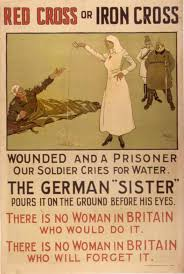
\includegraphics[width=0.32\linewidth]{images/redcross.jpg}
	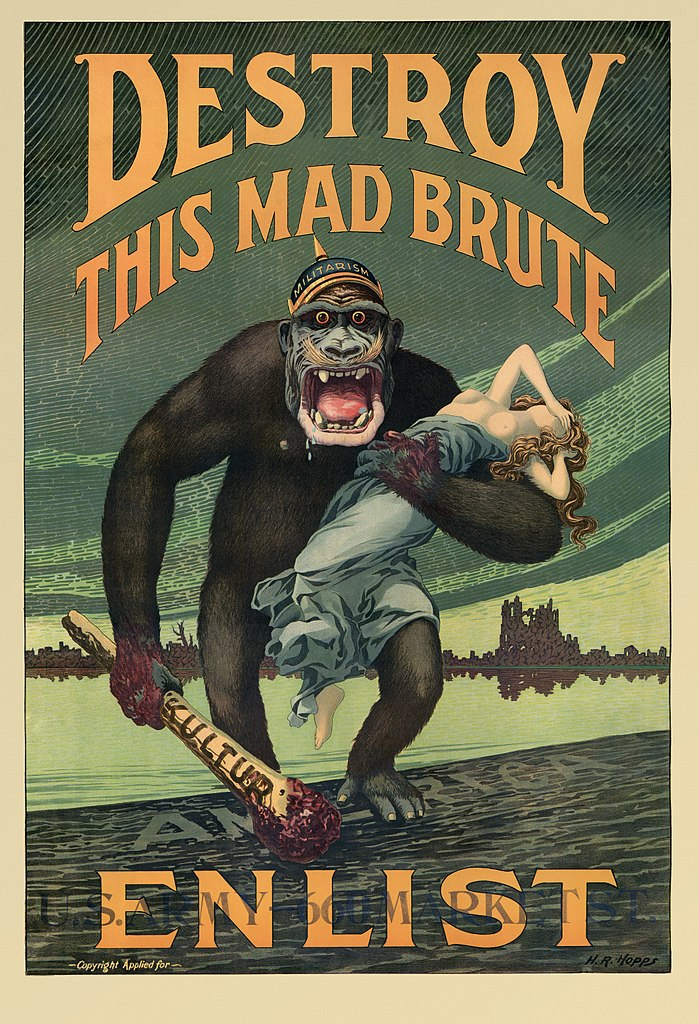
\includegraphics[width=0.32\linewidth]{images/hun1.jpg} % Figure image
	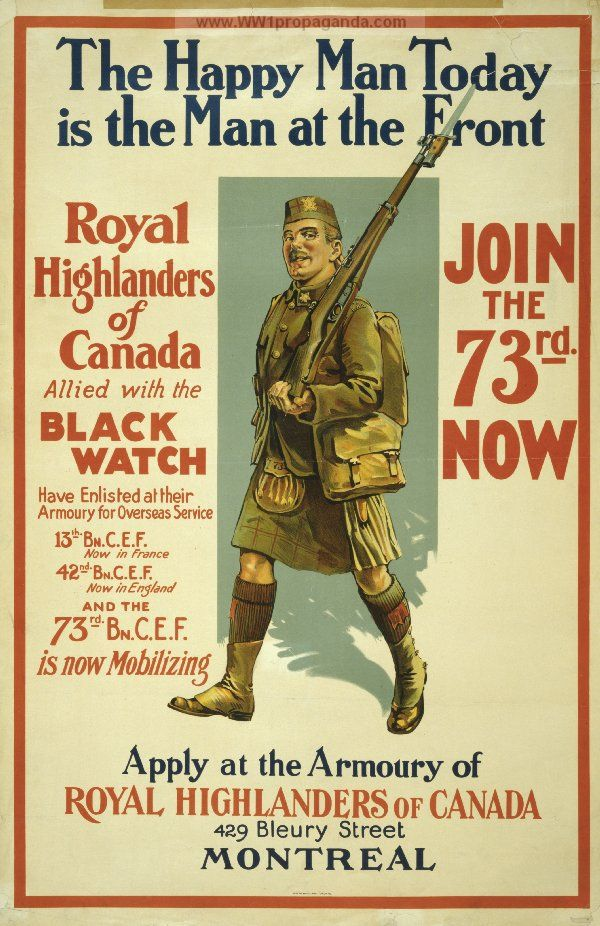
\includegraphics[width=0.32\linewidth]{images/happy.jpg}
	\caption{Various propaganda posters from WWI. They can either present an over negative image of the enemy or an over positive image of the own position (Imagine all the happiness you would feel, once you were at the WWI trenches at the front)} % Figure caption
	\label{FIG:WWI} % Label for referencing with \ref{bear}
\end{figure}
If one looks closely at the examples, it quickly becomes clear that they were issued by state actors that had control over the media and press. Nowadays the media landscape becomes much more fractured and either state actors can influence the media in other states (i.e. Russia buying Facebook ads in the US), or non-state actors can have a significant influence on the media (i.e. The Brexit campaign on Facebook). Also one does not need to control significant resources to start a new communication channel that can reach large parts of the population (i.e. youtube influencers, websites as infowars). So in short, the growth of importance of fake news is defined by the loss of influence of state actors and media on their own state, which is replaced by the growth of influence of non-state actors who's identity is often easily hidden and who can have an outsized influence on public opinion for the budget they have.
Independent of whether the fake news is created by traditional states, media or new non-state actors what are the ways in which it can be detected and fought? Fake news, especially in non-traditional media, needs to spread in order to effectively influence the public targeted. Research has show that people are much more likely to spread news in case it provokes anger or makes them feel good and confirms or strengthens existing biases and is easy to grasp. News that makes one feel sad, shamed, guilty or even jokes are much less spread. Especially news that sends a double message that is conflicting with ones own confirmation bias is much less likely to spread. This provides us several tools in which one can detect if a message was designed to be spread
\begin{itemize}
\item News that is unusual positive or unusually strong provoking anger are more likely to be designed to spread fake news.
\item News that uses more than usual simplified language (words or sentence construction), or is shorter than usual is more likely to contain fake news.
\item News containing many words statistically correlated with fake news are more likely to contain fake news
\item News written by authors that publish ofter than usual fake news are more likely to publish fake news.
\end{itemize}
Of course all measures are determined by \"more than usual\". One cannot expect the Guildford Evening Courrier\cite{adams1979} to have the same style, word choice and article length as Foreign Policy.
Finally statistically sampling for abnormal patterns can be very effective as shown by the use of Benfords law to detect accounting fraud. One can sample the words used an see if certain words are more likely to be used for faked news as for actual news.

One complicating factor is that fake news is often a sliding scale. Messages can be outright fabricated, but it much more common that part of the news is true but distorted or exaggerated or part of the facts are made up. For this reason we combine different detection techniques into a final score that tells how trustable we deem a news message. 

What makes fake news a more relavant topic than before, however is that before the main actors producing fake news were the state and the major publishers. However it has become more easy to spread fake news, while at the same time due to falling budgets news publishers have less budgets to fund their own research to verify the stories.
\begin{itemize}
\item Actors can easily hide their identity and one actor can impersonate many identities to spread the same message, making it appear that many actors are involved in spreading the news.
\item Actors can easily target large target populations through targeted adds on social media
\item Actors can pay people with a large following to spread their news.
\item Bots can easily make it appear that there is quite a buzz going on about a news item
\item We can not go and check ourselves, so we need to trust someone to tell us whether it was true or not.
\end{itemize}


\section{Definition of Fake News}
Fake news is a general term that is hard to pinpoint as it contains several uses. In order to get a clear understanding we look at the different uses and define it in each instance what it mean. Starting from the intended use we can more easily identify the techniques employed. 
\begin{itemize}
\item Group Identification. Obvious false facts to identify as group. A prime example is the US where mask wearing has been used to identify political inclinations instead of recognizing the obvious truth that it is beneficial for all people to wear a mask. In order to belong one needs to make belief.
\item Opponent Identification. Distorted facts to divide own public from the rest. An excellent example of this class is the statement that Black Live Matter protesters are looting scum. Which will of course drive a division between left and right.
\item Motivate Base. Distorted facts to convince own public and or allies. Examples of this are the gulf of Tonkin incident also the ``proof'' of Iraq owning nuclear weapons. 
\item Swing undecided. This a relatively minor aim as mostly opponents are not easily convinced. However it can be used to swing the opinion of undecided voters.
\item Distract and Redirect. Creating anger about an unrelated subject helps to deflect attention from the relevant facts.
\item Create Unrest. This allows for a strongman to step in. 
\end{itemize}  
From this we can develop the following definition of Fake News.
Fake news is an piece of information that.
\begin{itemize}
\item Is engineered to spread. This makes should make the news outstanding and evoke strong emotions (in particular anger and joy) \cite{vosoughi2018}.
\item It needs to be understood immediately, which require simple language with respect to the target group and not allow for nuances or partial truths.
\item It needs to create a clear distinction between opponents and proponents
\item It needs to be factually incorrect (i.e. engineered).
\end{itemize}

\begin{table}
	\caption{Different Uses of Fake News}
	\centering
	\begin{tabular}{llr}
		\toprule
		\multicolumn{2}{c}{Name} \\
		\cmidrule(r){1-2}
		Group Identification   & Believe to Belong &  \\
		                       & Division          &  \\
		                       & Identification    &  \\
                Opponent Identification & & \\
                Mobilize Base           & &  \\
		Influence Opinion       &  &  \\
		Distract \& Deflect     &   &  \\
		Create Unrest           &  &  \\
		\bottomrule
	\end{tabular}
\end{table}




\section{Theory of Fake News Detection}
Now that we have a definition of what fake news is we can identify the different points that distinguish it and use these to detect when a news item is fake \cite{zhou2020}.
\begin{table}
	\caption{Patterns to identify Fake News}
	\centering
	\begin{tabular}{llr}
		\toprule
		\multicolumn{2}{c}{Name} \\
		\cmidrule(r){1-2}
		Factual Checking       & Manual    & Experts  \\
		                       &           & Crowd Checking \\
		                       & Automatic & Predicate Testing \\
                Style                  & Quantity  & \\
                                       & Complexity & \\
                                       & Uncertainty & \\
                                       & Complexity & \\
                                       & Subjectivity & \\
                                       & Non-immediacy & \\
                                       & Diversity & \\
                                       & Specificity & \\
                Propagation            & Sentiment & \\
                                       & Emotional Content & \\
                                       & Distribution Channels & \\
                                       & Spread on Social Media (Retweets) & \\
                Source                 & Author & \\
                                       & Publisher & \\
                Correlation            & Words correlation & \\
                                       & Factual Similarities & \\
                                       & Source Similarities & \\
		\bottomrule
	\end{tabular}
\end{table}


\subsection{Factual Checking}
Fact checking is of course the most obvious way to assess whether news is fake. It is the most important way at the moment to determine if news was faked. However it also has sever drawbacks
\begin{itemize}
\item Fact Checking is labour intensive as it involves a significant amount of manual checking. Even the machine learning algorithms will require a significant input of manually checked facts. 
\item The facts needs to come from somewhere, which means one would either need to trust experts, or reference works. 
\item As seen in the introduction fake news can be about the way facts are represented. So even though the content might be true they may be place into a context that misrepresents the facts.
\end{itemize}
Currently at bywire we are using fact checking only on an ad-hoc basis. The core algorithm comprises of indicators that can be easily employed on a statistical basis.

\subsection{Style Checking}
Style checking is an important indicator
\begin{table}
	\caption{Style Elements to identify Fake News}
	\centering
	\begin{tabular}{llr}
		\toprule
		\multicolumn{2}{c}{Name} \\
		\cmidrule(r){1-2}
		Quantity       & Character Count &  \\
		               & Word Count      &  \\
		               & Noun Count      &  \\
		               & Verb Count      &  \\
		               & Number of noun phrases &  \\
		               & Sentence Count  &  \\
		               & Paragraph Count &  \\
		               & Modifier Count (Adjectives/Adverbs/...) &  \\
		 Complexity    & Avg. Number of clauses per sentence     &  \\
		               & Avg. Number of words per sentence       &  \\
		               & Avg. Number of characters per word      &  \\
		               & Avg. Number of punctuation per sentence &  \\
		 Uncertainty   & Percentage of modal verbs               &  \\
		               & Percentage of certainty terms           &  \\
		               & Percentage of generalizing terms        &  \\
		               & Percentage of tentative terms           &  \\
		               & Percentage of numbers and quantifiers   &  \\
		               & Number of question marks                &  \\
		 Subjectivity  & Percentage of subjective verbs          &  \\
		               & Percentage of report verbs              &  \\
		               & Percentage of factive verbs             &  \\
		               & Percentage of imperative commands       &  \\
		 Nonimmediacy  & Percentage of passive voice             &  \\
		               & Percentage of rhetorical questions      &  \\
		               & Self reference: 1st person pronouns     &  \\
		               & Group reference: 1st per. plural pronouns &  \\
		               & Other reference: 2, 3 per. pronouns     &  \\
		               & Number of quotations                    &  \\
		               & Number of exclamations marks            &  \\
		               & Activation: dynamics of emotional state &  \\
		 Diversity     & Lexical diversity (unique words)        &  \\
                               & Content word diversity                  &  \\
                               & Reduncancy                              &  \\
                               & Informality Typographical error ratio   &  \\
                 Specificity   & Temporal Ratio                          &  \\
                               & Spatial Ratio                           &  \\
                               & Sensory Ratio                           &  \\
                               & Causation Terms                         &  \\
                               & Exclusive Terms                         &  \\
                               & Readability (Flesch-Kincaid/Gunning-Fog) &  \\
		\bottomrule
	\end{tabular}
\end{table}

\subsection{Correlation}
In order for fake news to be more effective the same message is repeated often in different forms.
Also certain terms are more likely to provoke a strong response. At ByWire we use the following measures
\begin{itemize}
\item Dictionary with known correlation with fake news per word and word group. This dictionary is improved upon over time.
\item Correlation with other articles in the bywire database.
\item Correlation with other articles on the internet.
\item Correlation with other articles by the same source (This is treated in the source section).
\end{itemize}

\begin{table}
	\caption{Patterns to identify Fake News}
	\centering
	\begin{tabular}{llr}
		\toprule
		\multicolumn{2}{c}{Name} \\
		\cmidrule(r){1-2}
		Factual Checking       & Manual    & Experts  \\
		                       &           & Crowd Checking \\
		                       & Automatic & Predicate Testing \\
                Style                  & Quantity  & \\
                                       & Complexity & \\
                                       & Uncertainty & \\
                                       & Complexity & \\
                                       & Subjectivity & \\
                                       & Non-immediacy & \\
                                       & Diversity & \\
                                       & Specificity & \\
                Propagation            & Sentiment & \\
                                       & Emotional Content & \\
                                       & Distribution Channels & \\
                                       & Spread/Retweets & \\
                Source                 & Author & \\
                                       & Publisher & \\
                Correlation            & Words correlation & \\
                                       & Factual Similarities & \\
                                       & Social Media Pickup & \\
                                       & Source Similarities & \\
		\bottomrule
	\end{tabular}
\end{table}



\subsection{Propagation}
An essential facet of fake news is that it is propagated to reach a significant audience. A perfectly engineered message is useless when it doesn't arrive at the target audience. At bywire we distinguished the following means to engineer propagatin \cite{vosoughi2018}, \cite{sivek2019}.
\begin{itemize}
\item Messages provoking strong feelings of Anger and Trust
\item Number of shares / retweets.
\item Language used (this is taken care of by the style indicator).
\item Number of search results when searching for the message text.
\end{itemize}

\begin{table}
	\caption{Patterns to identify Fake News}
	\centering
	\begin{tabular}{llr}
		\toprule
		\multicolumn{2}{c}{Name} \\
		\cmidrule(r){1-2}
		Factual Checking       & Manual    & Experts  \\
		                       &           & Crowd Checking \\
		                       & Automatic & Predicate Testing \\
                Style                  & Quantity  & \\
                                       & Complexity & \\
                                       & Uncertainty & \\
                                       & Complexity & \\
                                       & Subjectivity & \\
                                       & Non-immediacy & \\
                                       & Diversity & \\
                                       & Specificity & \\
                Propagation            & Sentiment & \\
                                       & Emotional Content & \\
                                       & Distribution Channels & \\
                                       & Spread/Retweets & \\
                Source                 & Author & \\
                                       & Publisher & \\
                Correlation            & Words correlation & \\
                                       & Factual Similarities & \\
                                       & Social Media Pickup & \\
                                       & Source Similarities & \\
		\bottomrule
	\end{tabular}
\end{table}



\subsection{Source}
One of the most important distinguishing factors in fake news detection is the source \cite{sitaula2019}. This is something one knows intuitively, as one is likely to trust the Times more than Cosmopolitan. However this does not mean one is less likely to read Cosmopolitan. Since it depends also strongly on the topic (i.e. Cosmopolitan over the Times for celebrity gossip). At ByWire we implemented the following algorithm.
\begin{itemize}
\item For each source (newspaper and writer) calculate an overall score and an topic score based for all articles published.
\item Calculate a score per topic.
\item For each channel (twitter, site, facebook) calculate an overall score and an topic score based for all articles published.
\item For authors combine the different papers for which they write in such a way that most discerning power is obtained.
\item Combine each score in a way that adds most discerning power.
\end{itemize}


\section{Methodology}
The algorithm to detect fake news a bywire was constructed using standard data science techniques. First a training and test set were developed using manually labelling fake and non-fake messages. Based on this test set 
\begin{itemize}
\item Optimize the coefficients of each individual measure.
\item Determine of each individual measure whether it has predictive power to discern between fake news and factual news.
\item Test on test data to see if the predictive power holds up.
\item Calculate a score per category to determine which elements of a fake news message are pronounced.
\item Combine the individual measures to improve the predictive power.
\item Test on test data to see if the predictive power holds up.
\item Test on out of sample data to validate that the constructed model is stable and not an artifact of the dataset (overfitting).
\end{itemize}

\section{Results}




%	BIBLIOGRAPHY
%----------------------------------------------------------------------------------------

\printbibliography[title={Bibliography}] % Print the bibliography, section title in curly brackets




%----------------------------------------------------------------------------------------

\end{document}
